
    \begin{picture} (170.000000,128.000000)(0,0)
    \put(0.0, 0.0){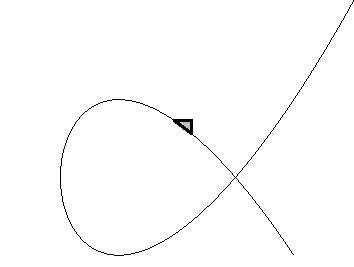
\includegraphics{09arclength-Leibniz.pdf}}
        \put( 79.88,  61.18){\sffamily\itshape $ds$}
    \put( 87.94,  73.18){\sffamily\itshape \makebox[0pt][c]{$dx$}}
    \put( 95.00,  65.09){\sffamily\itshape \makebox[0pt][l]{$dy$}}
\end{picture}
